\subsection{Critical Temperature and Conviction Buildup}\label{sec:results_temperature}

\begin{figure}[t]
    \centering
    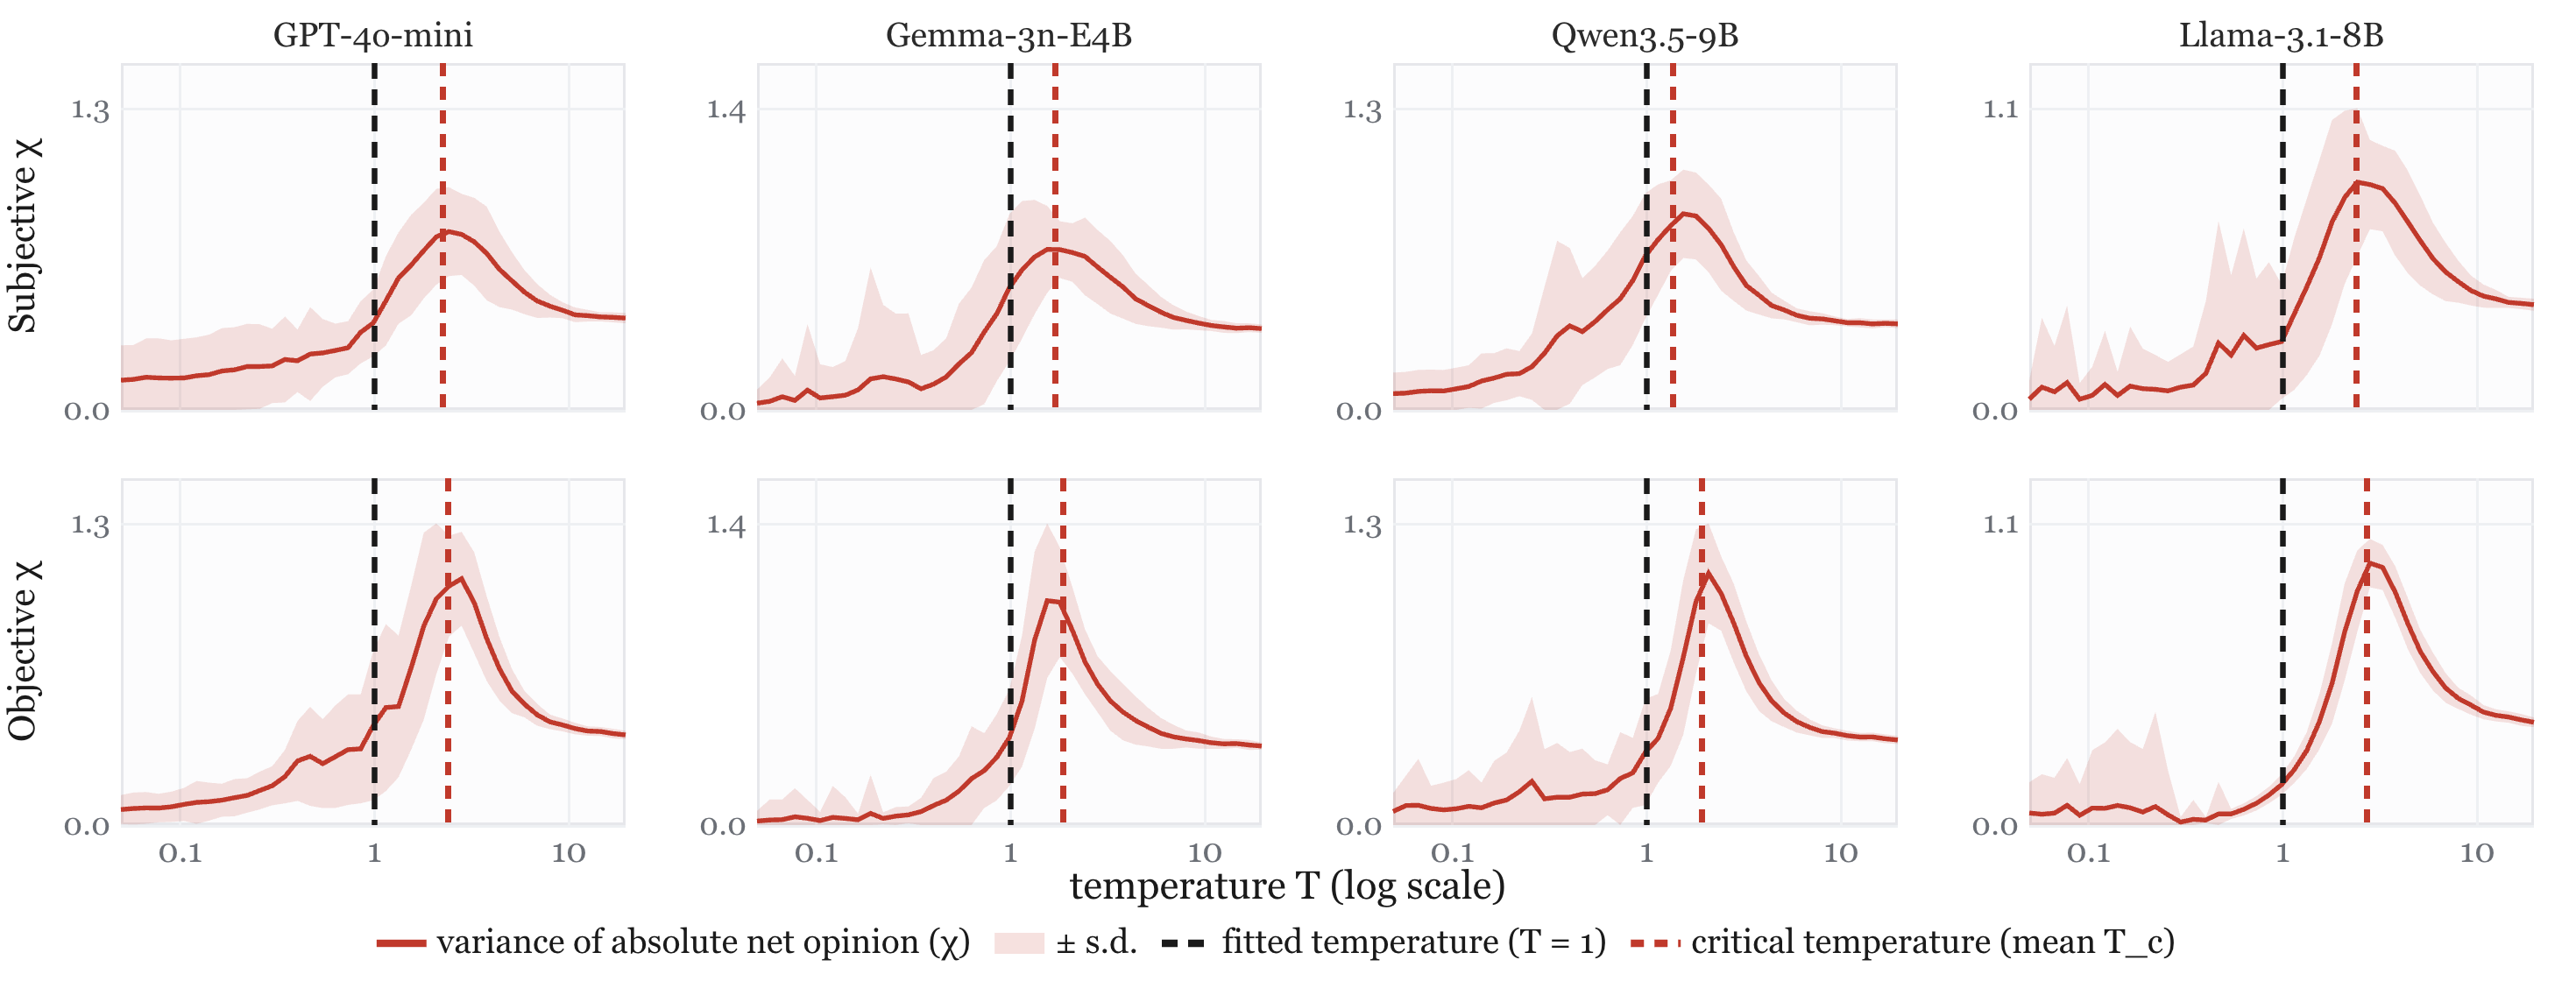
\includegraphics[width=0.99\textwidth]{main/Figures/main_07_critical_temperature.png}
\caption{\textit{Critical temperature.} 
Variance of absolute net opinion $\chi$, whose peak gives the critical temperature $\mathcal{T}_c$ for each community. Individual communities are reported in Figure \ref{fig:agent_model_tc_mean_test_J03_fitted_nomf_tcmean_qea} from  Appendix \ref{apdx:per_society_transitions}. Here we report instead the mean of the community critical temperatures $T_c$. 
The bold black dashed line is the fitted operating point $\mathcal{T}=1$ of the three coupling model. Every question from the held-out test questions evaluated on the $4$ in-distribution random test graphs (each of the $4$
graphs of the family $\times$ the questions, $20$ objective / $10$ subjective
questions).\label{fig:agent_model_tc_mean_test_J03_fitted_nomf_tcmean}}
\end{figure}

In Section \ref{sec:obs_phase_char}, we saw that conviction goes up over rounds and communities end up mostly in consensus or polarization. In statistical mechanics, whether a system stays ordered depends on where its temperature stands compared to the critical temperature. In this section, we introduce a temperature parameter into our model and check where our fitted communities sit relative to the critical temperature.
In Figure \ref{fig:agent_model_tc_mean_test_J03_fitted_nomf_tcmean}, we reintroduce a temperature parameter to examine our model’s behavior under different temperatures. The fitted-model rollouts use temperature $\mathcal{T}=1$. We explore 41 log-spaced temperature values from 0.05 to 20. We initialize each rollout using the community’s initial opinions at $t=0$ and apply the fitted rule for $500$ steps. Details of the experiment are discussed in Appendix \ref{apdx:per_society_transitions}.

\textit{Variance of Absolute Net Opinion.} We plot the  variance of the absolute net opinion scaled by the number of agents, $\chi$ for different temperatures $\mathcal{T}$.\footnote{In this experiment, we set $K=1$, hence, $o_i(t) = \bar{o}_i(t) = s_i(t)$ and $n(t) = \frac{1}{N}\sum_i \bar{o}_i(t) = \frac{1}{N}\sum_i s_i(t)$.}
$$\chi \;=\; N\,\mathrm{Var}_t\big(|n(t)|\big)$$
It records how much the net opinion moves throughout the rollout. At high $\mathcal{T}$ each agent follows noise, so the net opinion stays near zero at every step and barely moves. At low $\mathcal{T}$ the community is locked into one arrangement, so the net opinion is large but again barely moves. $\chi$ is small in both cases and large only in between.

\textit{Critical Temperature.} We take each community's critical temperature $\mathcal{T}_c$ to be the temperature at which $\chi$ peaks. This peak marks a transition: it is the temperature at which the community is undecided between the two behaviors described above. On either side, the net opinion is stable, either near zero (indifference) or near its ordered value by the couplings (consensus or polarization). At the critical temperature, it can swing between them. This critical temperature marks a finite-size analogue of a phase transition between the high conviction regimes (polarization and consensus) and the low conviction regime (indifference).\footnote{A phase transition in physical terms exists when $N \rightarrow \infty$.}   

\textit{Conviction Build-up.} Figure~\ref{fig:agent_model_tc_mean_test_J03_fitted_nomf_tcmean} shows that the fitted operating point lies below the critical temperature in every dataset--model cell. Below $\mathcal{T}_c$, the indifferent states are unstable. One way to understand this is that aligned neighbors raise an agent's local field, so an agent that agrees with its neighbors is unlikely to move out of its current position when there is low stochasticity. Thus, the model predicts that conviction grows over rounds rather than fluctuating, as observed in Section~\ref{sec:obs_phase_char}.
